\documentclass[a4paper, 12pt]{report}
\usepackage{mwe}
\usepackage{hyperref}


% \title{CE-321L/CS-330L: Computer Architecture}
% \subtitle{}
% \author{Syed Arsalan\\Syed Muhammad Ather Hashmi\\Syed Mujtaba Hassan\\ Habib University\\}



\begin{document}
\begin{titlepage}
	\centering

	{\Large \textsc{CE-321L/CS-330L: Computer Architecture}\par}
	\vspace{1.5cm}
	{\huge\bfseries Project Report\par}
	\vspace{2cm}
    {\Large\itshape Muhammad Arsalan Hussain\par}
    {\Large\itshape Muhammad Hashim Memon \par}
	{\Large\itshape Syed Muhammad Ather Hashmi\par}
    {\Large\itshape Syed Mujtaba Hassan\par}
    
    \vspace{1cm}
    {\large \today\par}
    \vspace{2cm}
    {\large{Habib University} \par}
    \par\vspace{1cm}
    
\includegraphics[scale = 0.8]{uhulogo.jpg}
    
	
	
	% \vfill

	% \vfill

% Bottom of the page
	
\end{titlepage}

% \maketitle
\section*{Introduction}
In this project we make a pipelined RISC-V processor, in verilog. 
We then wrote a code for the insertion sort algorithm and test ran that code on our processor.
We also ran it on a single cycle processor that we made and compared the results.
% • State your problem statement here and define your objectives
\section*{Methodology and Results}
% • Explain the project task wise.
% • Briefly describe the process of designing, the changes in code, snippets of the working or
% intermediate simulation (block diagrams, etc. are encouraged)
The project was divided into three tasks. In the first task we wrote the insertion sort algorithm in RISC-V assembly. 
We then converted it into machine code and ran it on our single cycle processor. The folowing are the code snippets of our insertion sort in RISC-V assembly
\\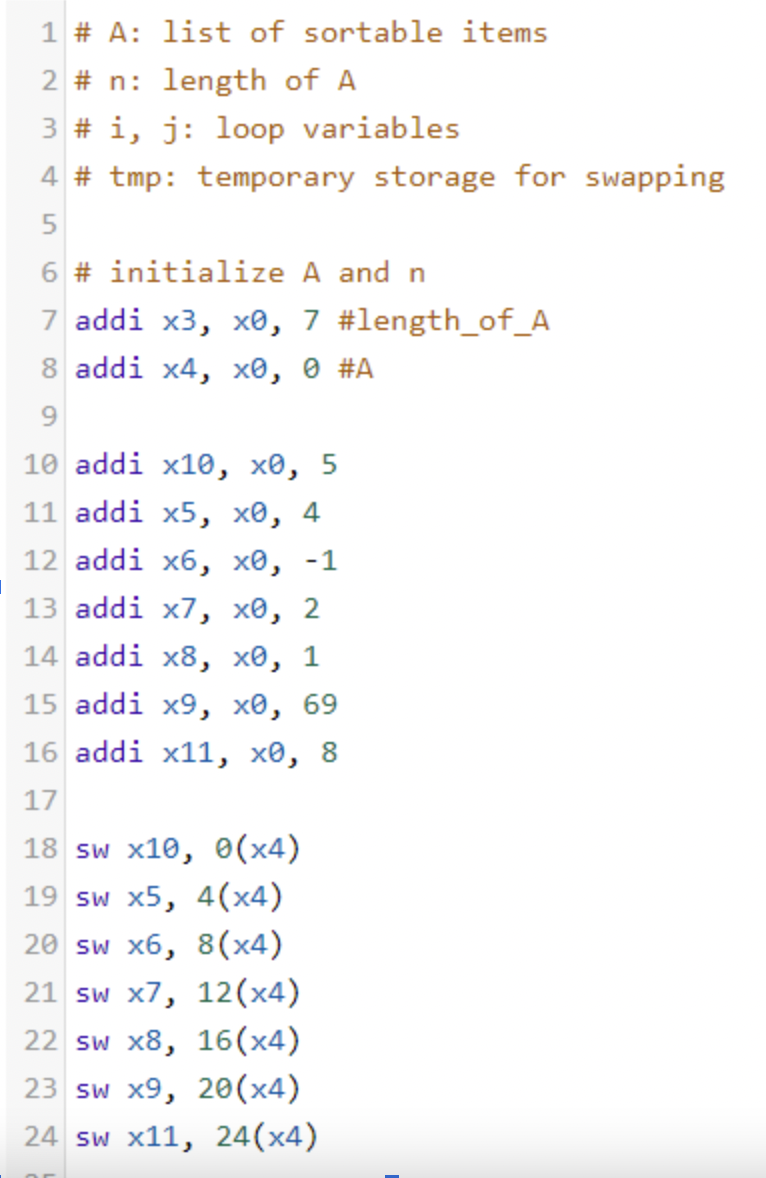
\includegraphics[scale = 0.5]{is1.png}
\\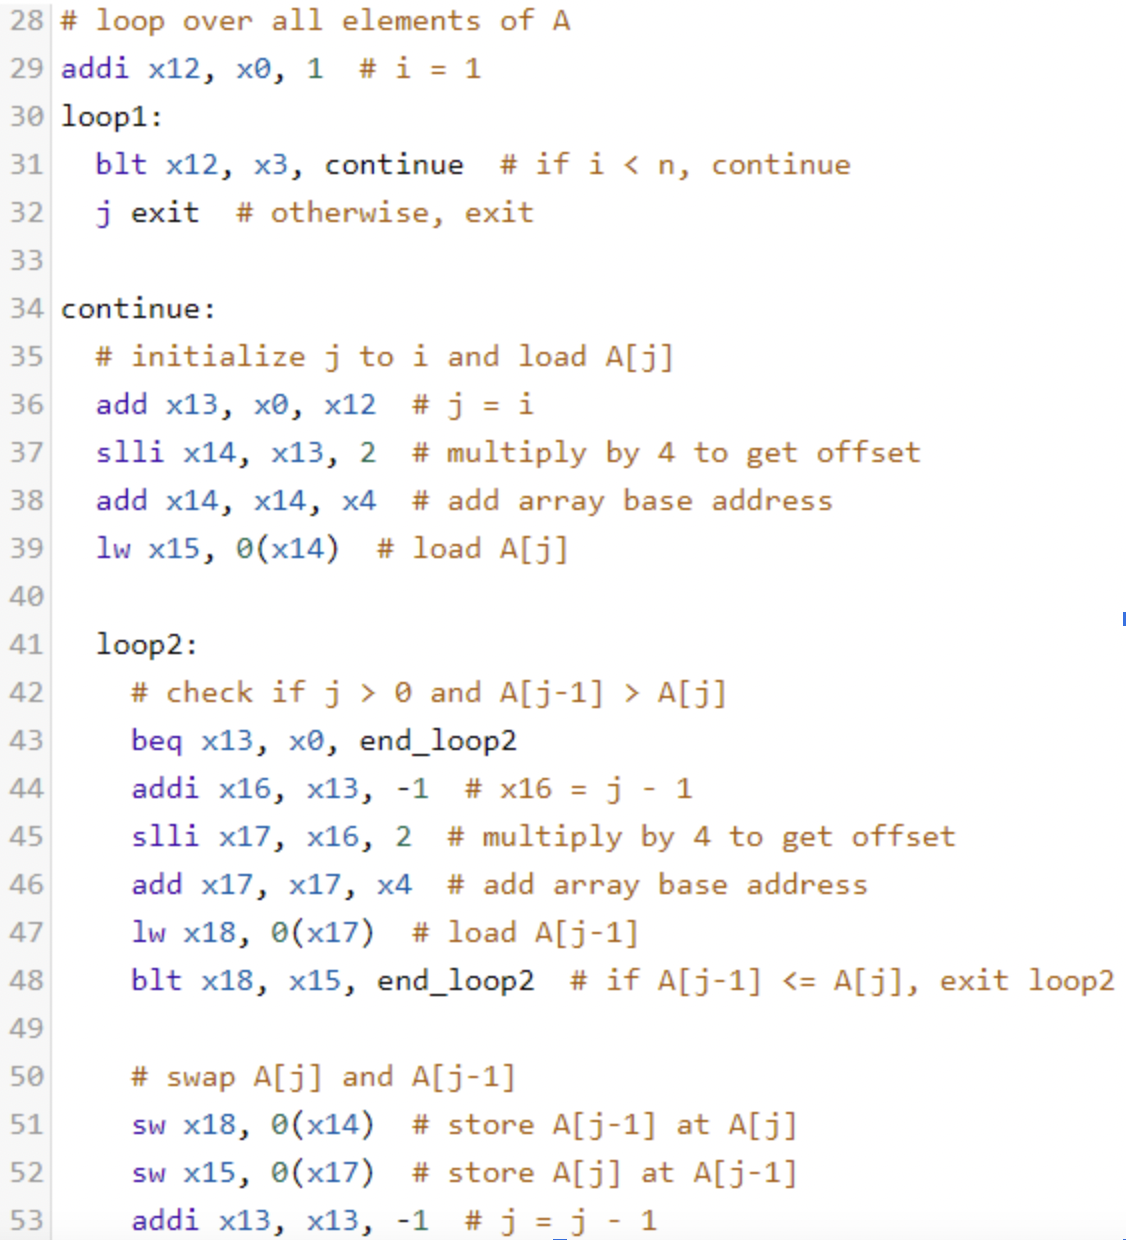
\includegraphics[scale = 0.5]{is2.png}
\\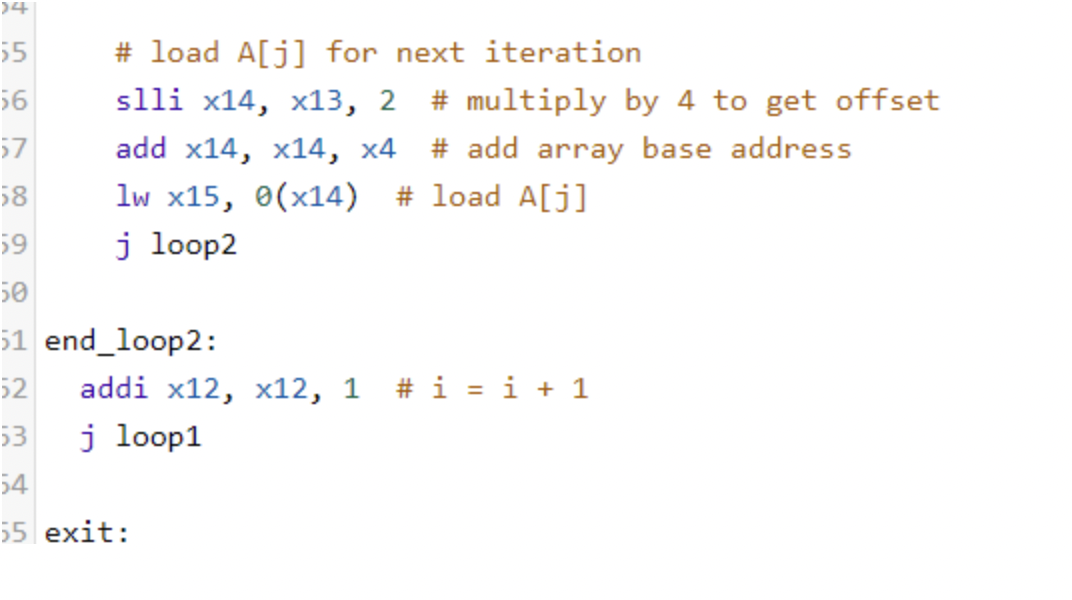
\includegraphics[scale = 0.5]{is3.png}
\\Following is the machine code equivalent of this code
\\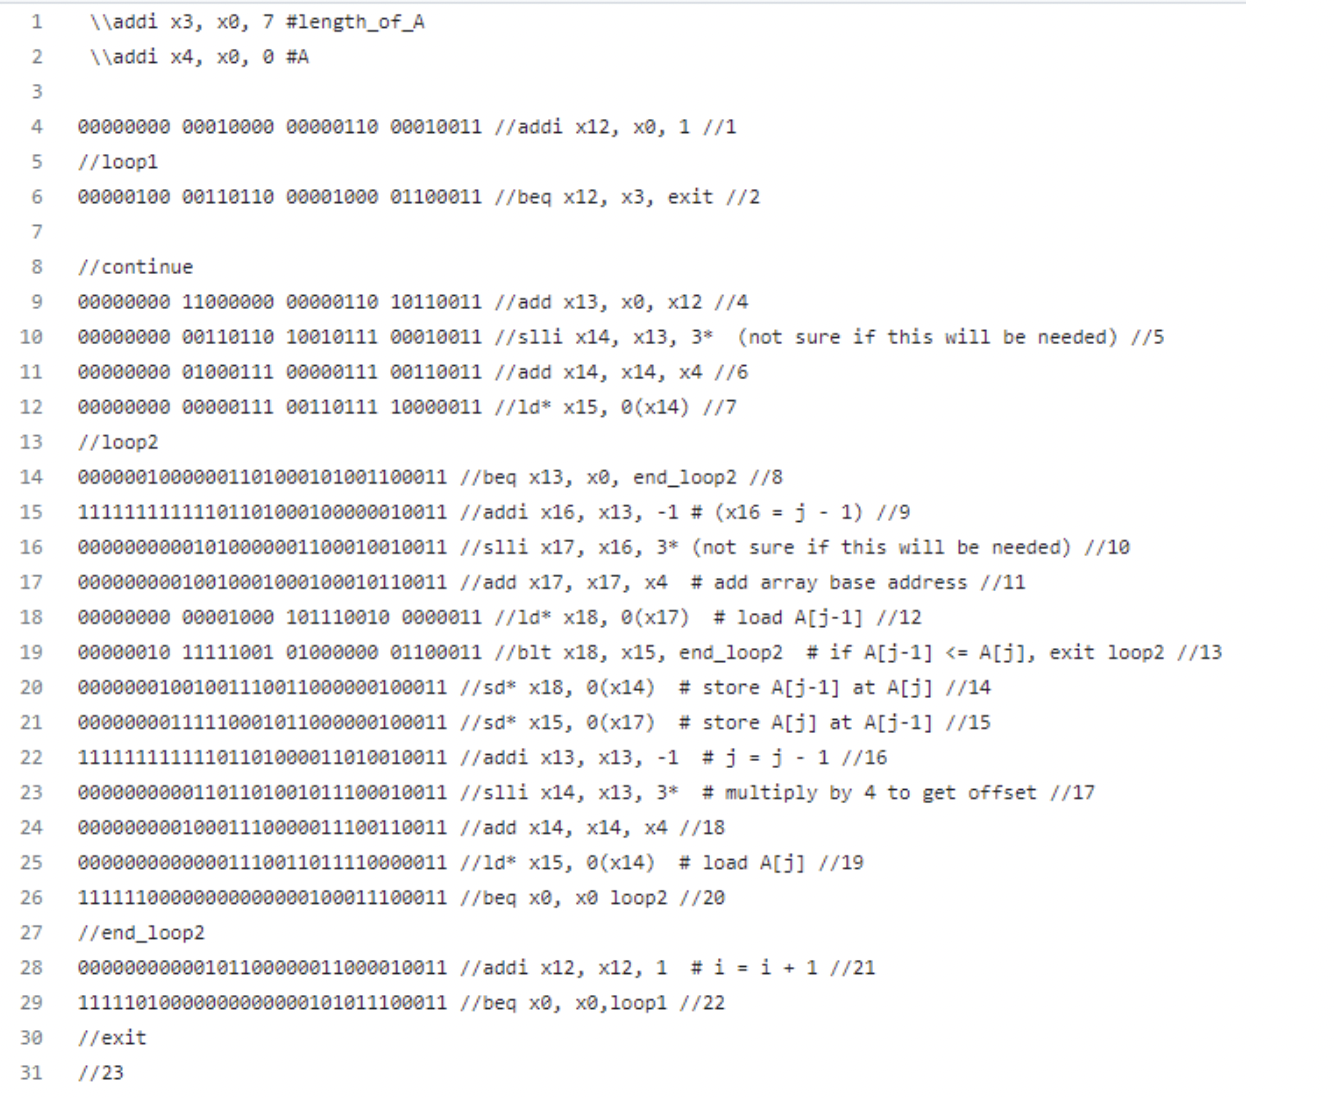
\includegraphics[scale = 0.5]{mc.png}
\pagebreak
\\The design of the top level module of the single cycle processor was taken from the book "Computer Organization and Design by David A. Patterson and John L. Hennessy".
The following code snippets shows the implementing of the top module of the single cycle processor:
\\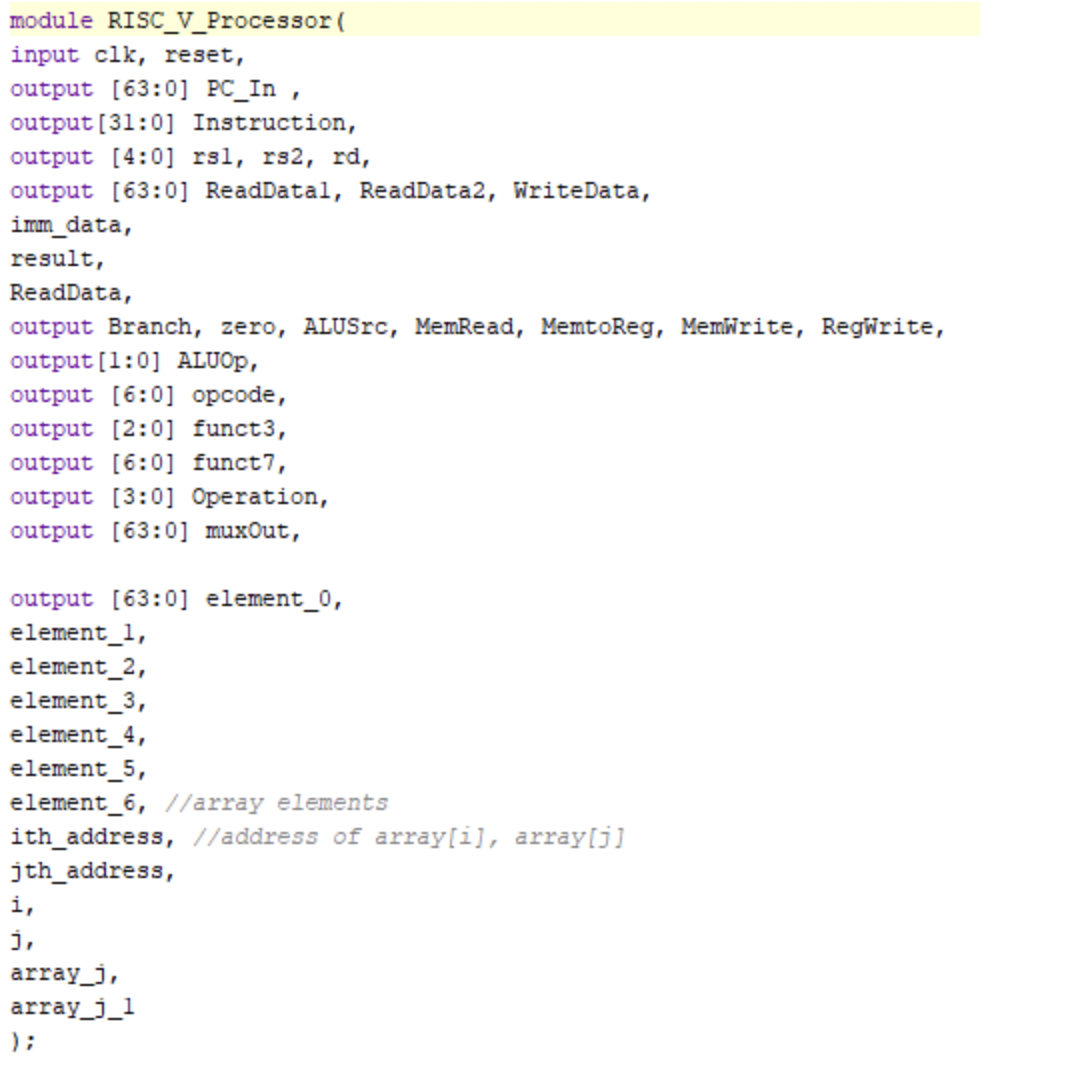
\includegraphics[scale = 0.5]{sc top 1.png}
\\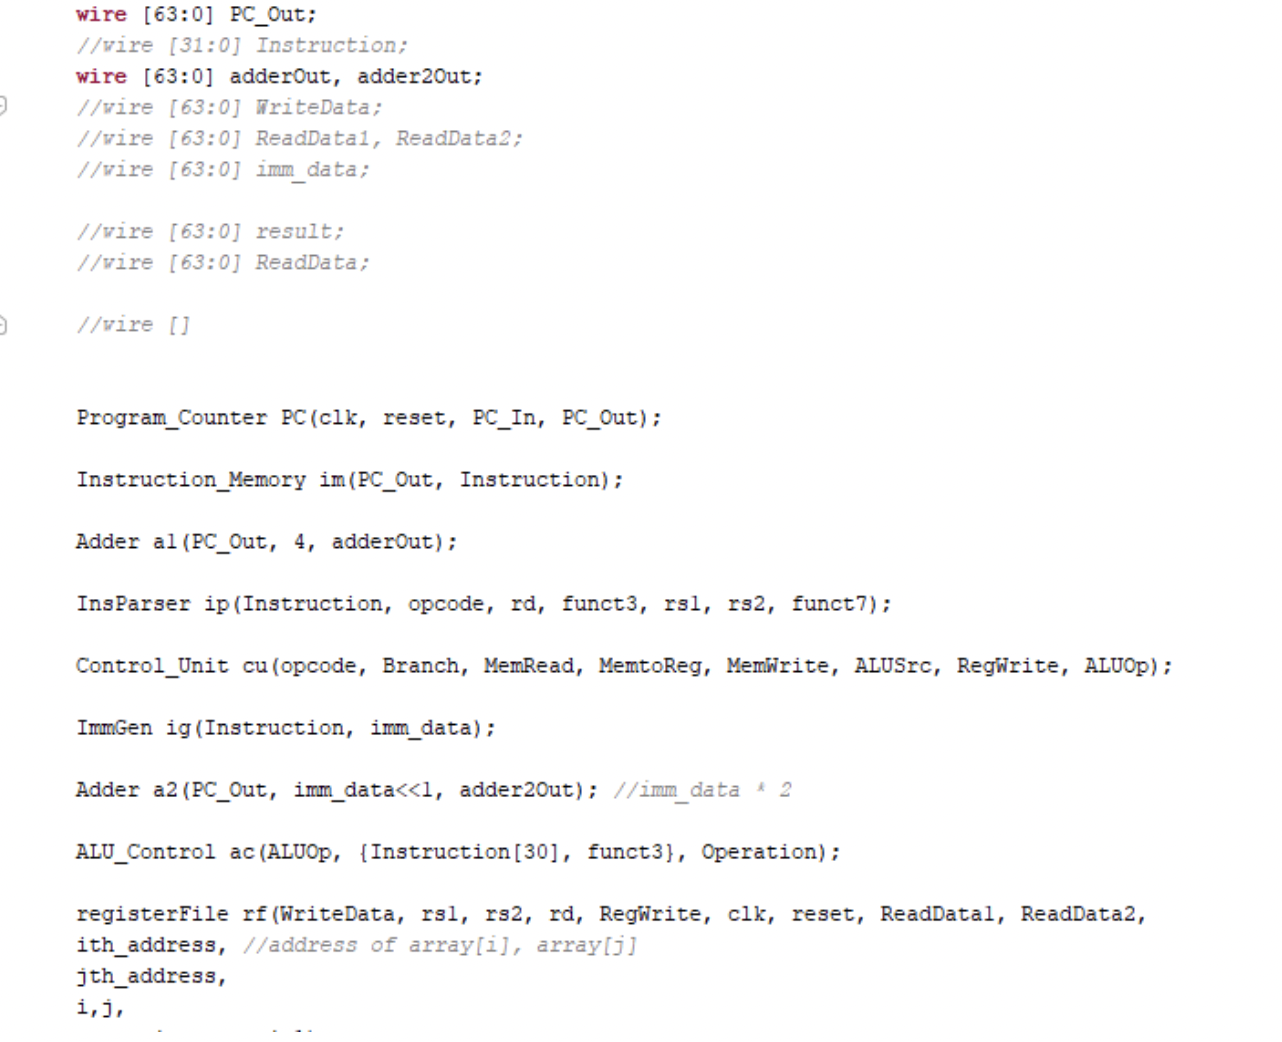
\includegraphics[scale = 0.5]{sc top 2.png}
\\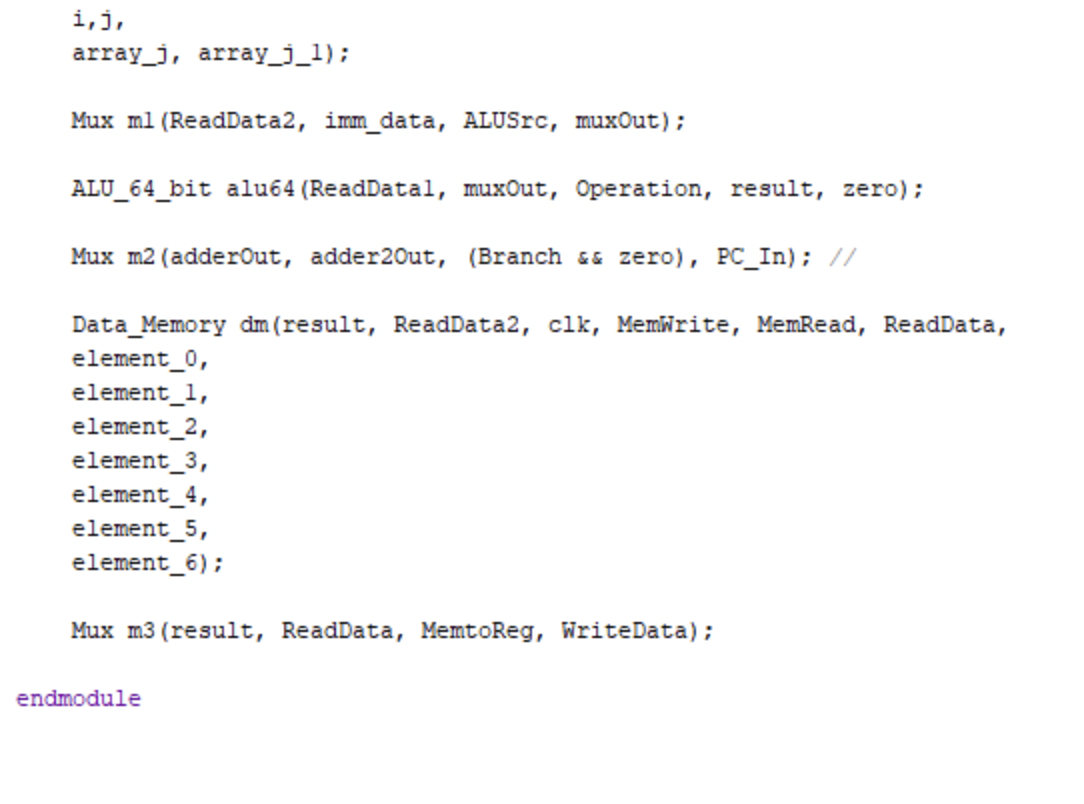
\includegraphics[scale = 0.5]{sc top 3.png}
\\The test module was written as follows
\\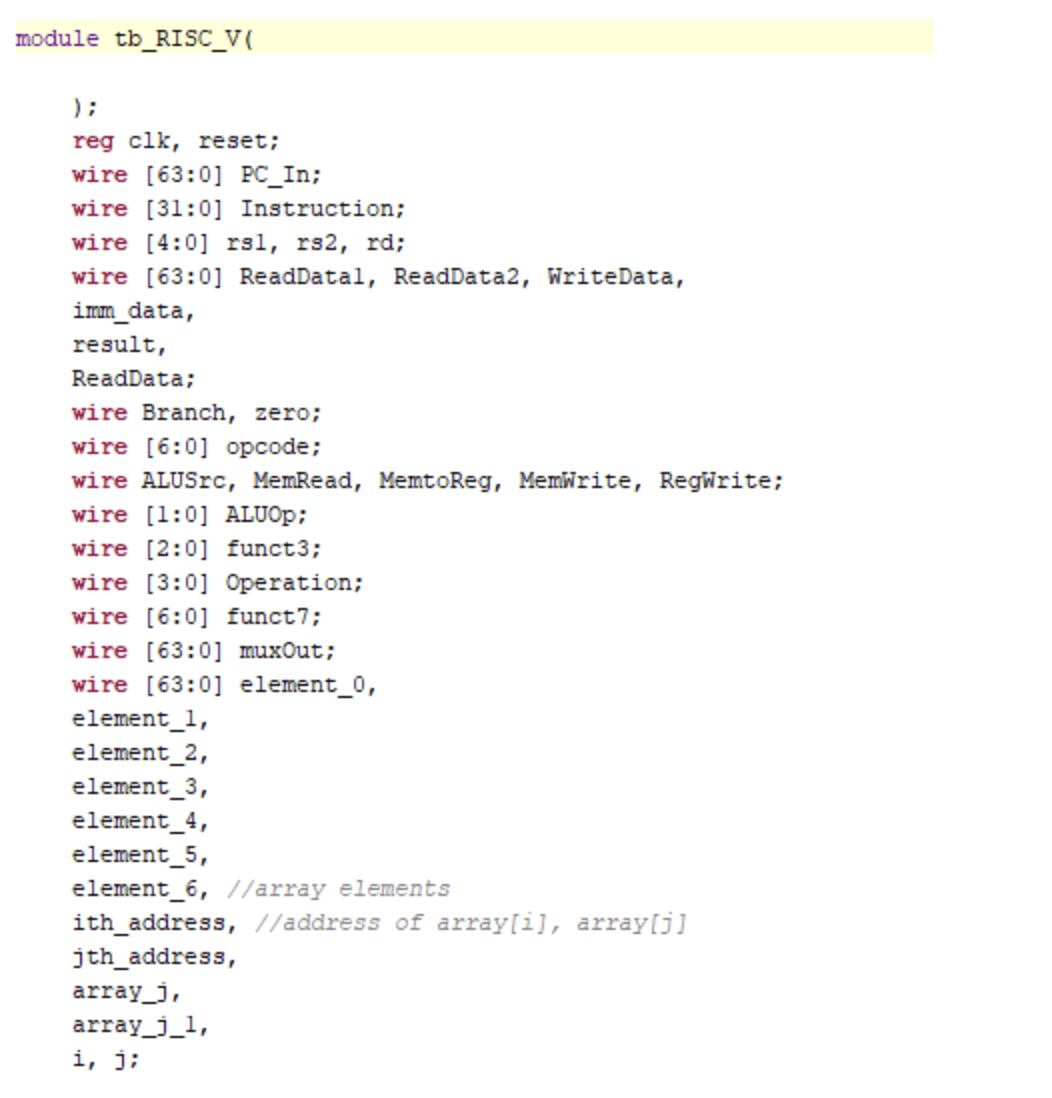
\includegraphics[scale = 0.5]{sc test 1.png}
\\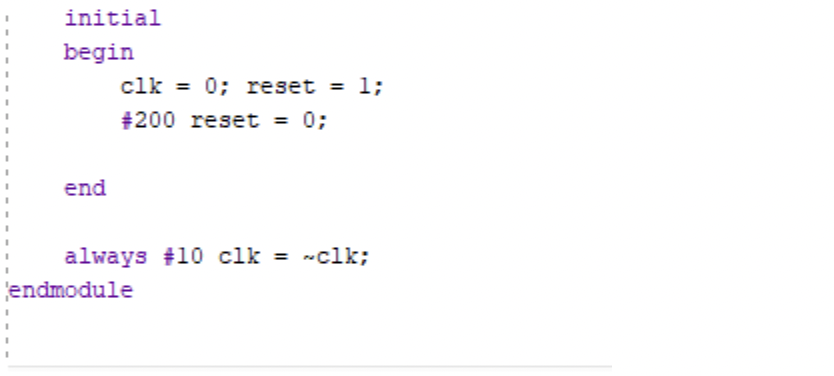
\includegraphics[scale = 0.5]{sc test 2.png}
\\With this the following EP waves were generated:
\\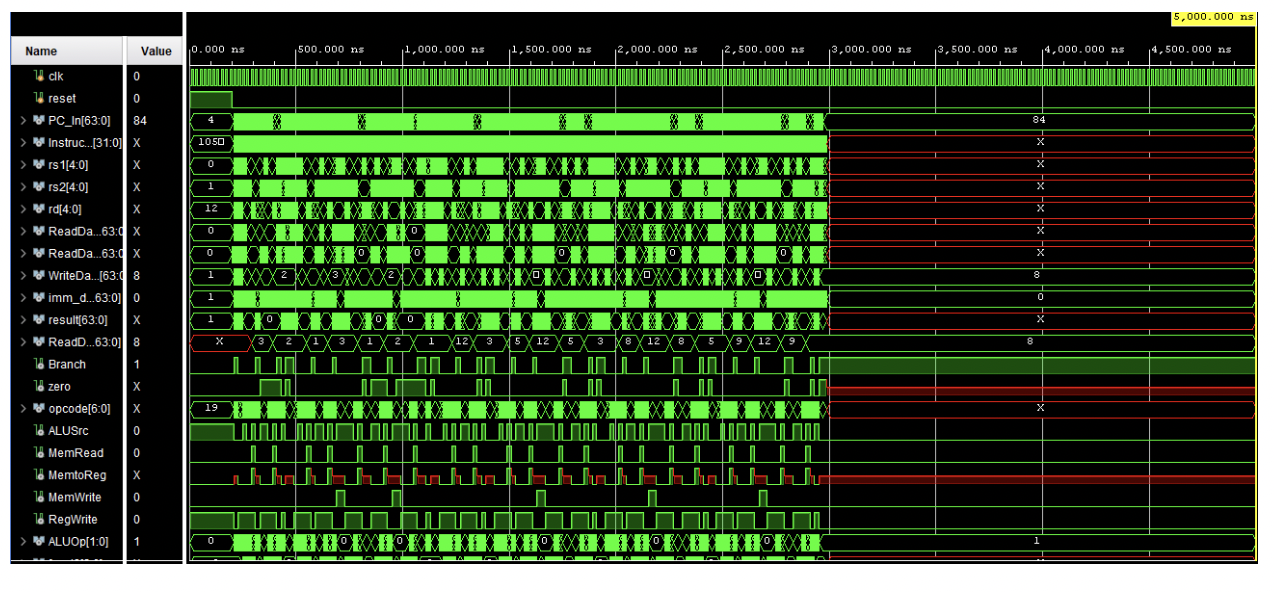
\includegraphics[scale = 0.5]{sc ep 1.png}
\\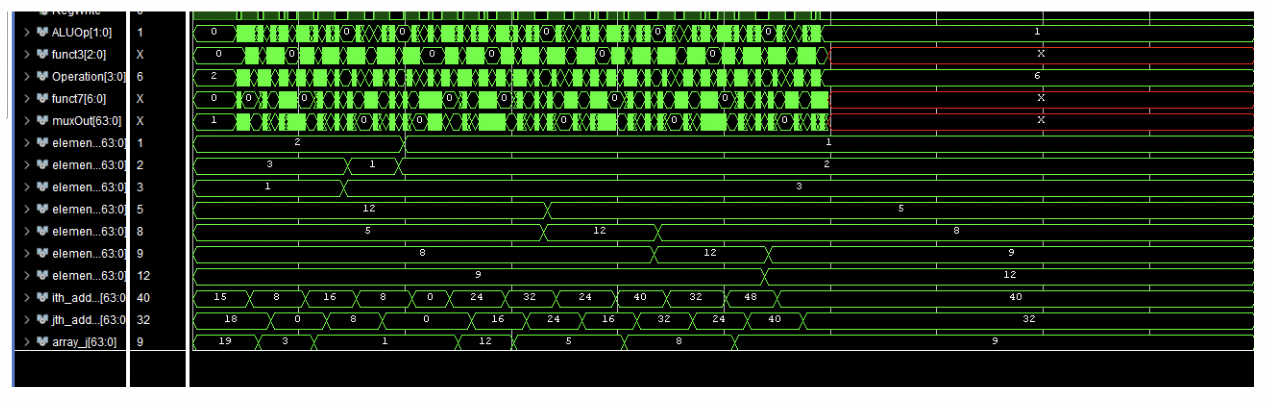
\includegraphics[scale = 0.5]{sc ep 2.png}
\\As you can see the single cycle processor works just fine and we get the correct results.
\\The code for Intermediate Modules can be found in the appendix.
\vspace{2cm}
\\The next task was to create a pipelined version of this processor. We again took the design from the book "Computer Organization and Design by David A. Patterson and John L. Hennessy".
\\We modified our single cycle processor to a pipelined version, then we ran and tested each instruction seperately to see if the pipeline can handle a single instruction.
\\We then added a hazard detetiong and  a forwarding unit to our pipelined processor and the next task was to test if the processor can run the entire sorting algorithm in this pipelined version
The following is a code snippet of the top module of the pipelined processor:
\\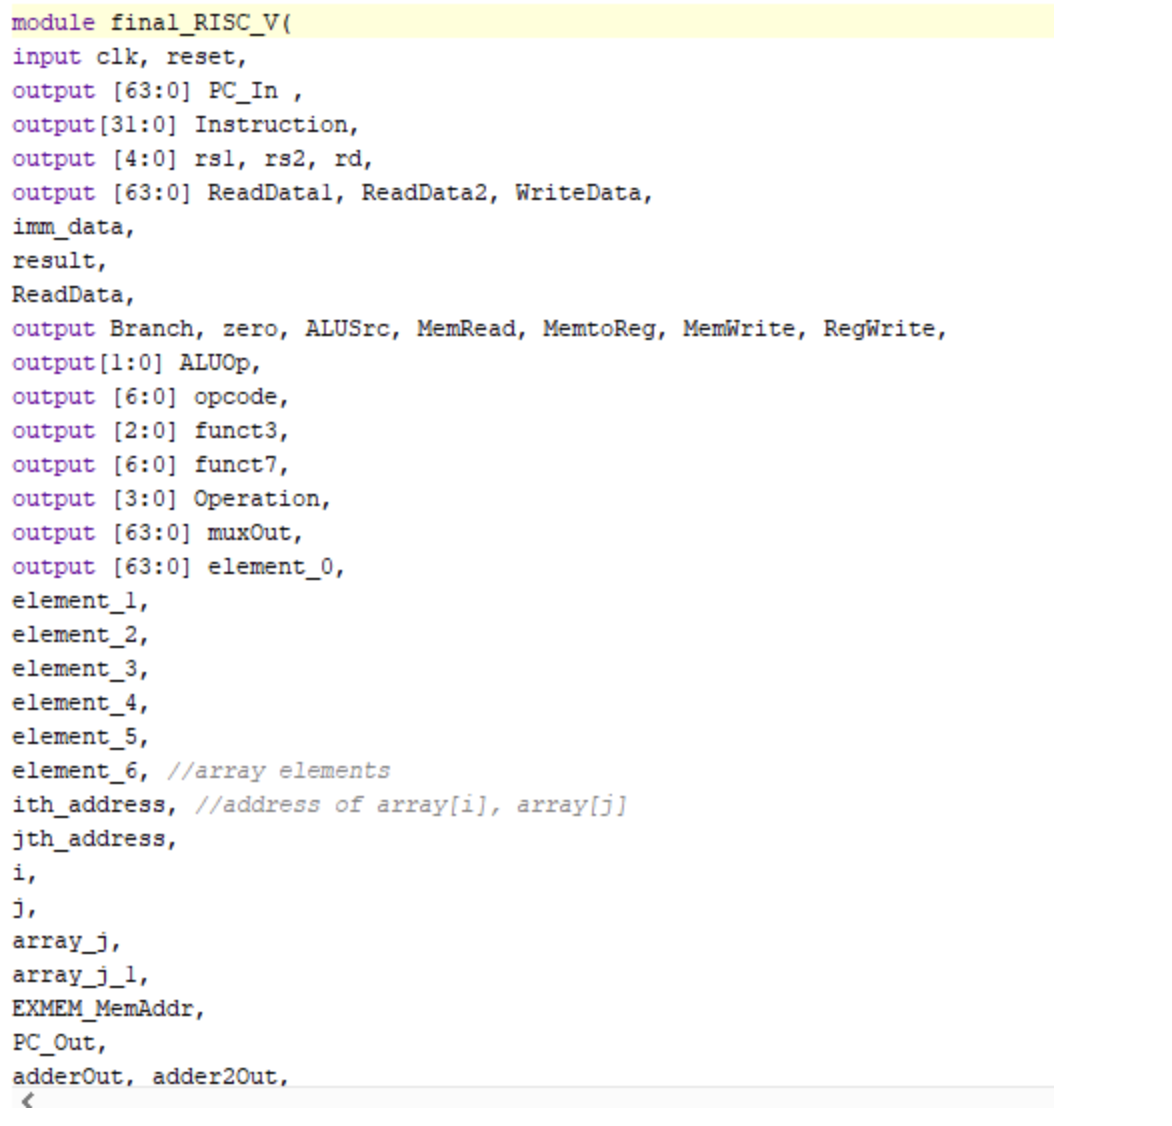
\includegraphics[scale = 0.5]{pipe top 1.png}
\\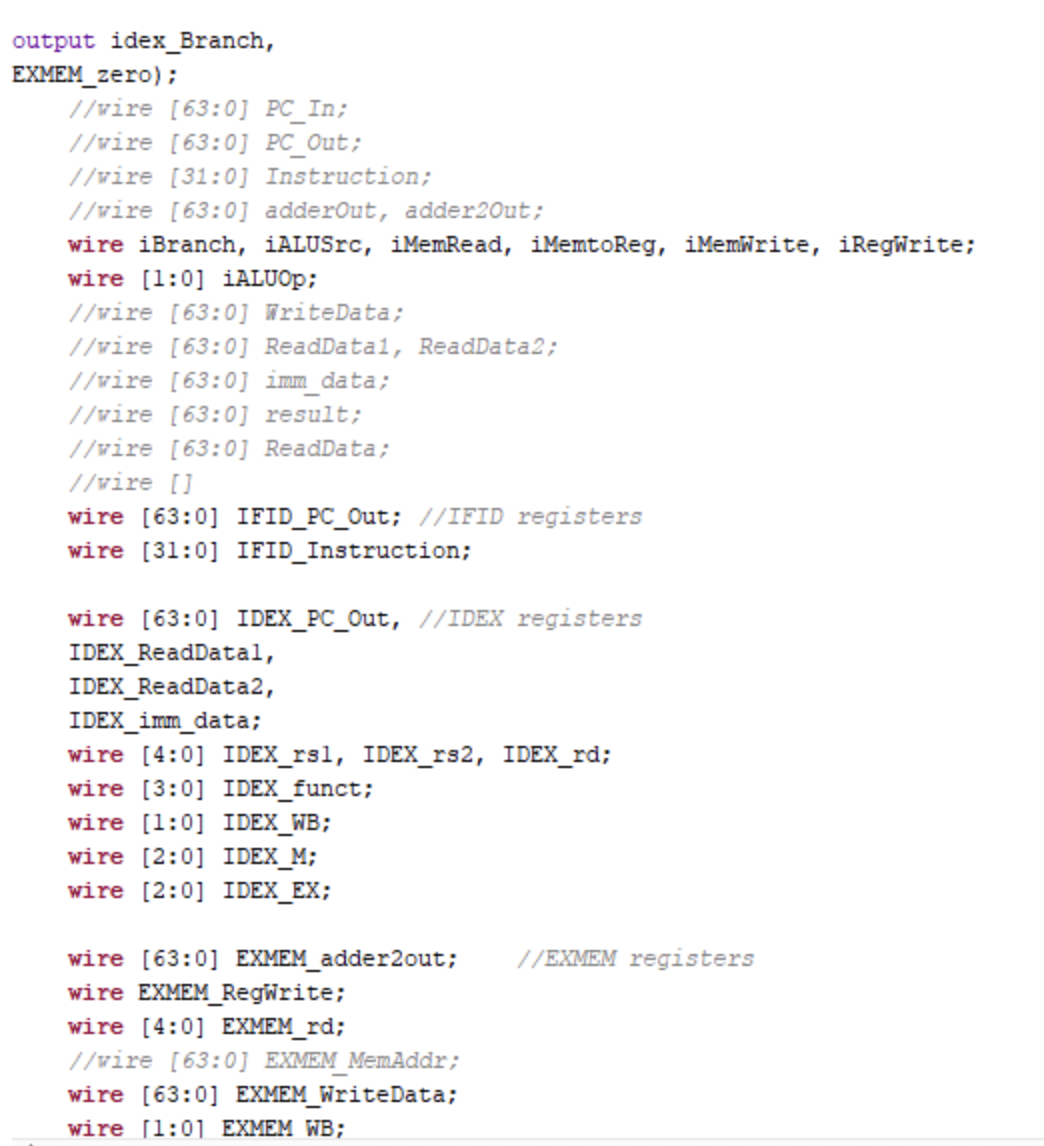
\includegraphics[scale = 0.5]{pipe top 2.png}
\\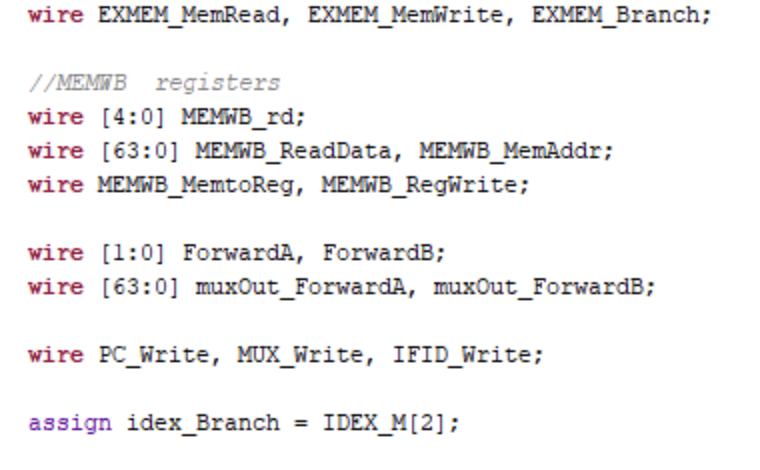
\includegraphics[scale = 0.5]{pipe top 3.png}
\\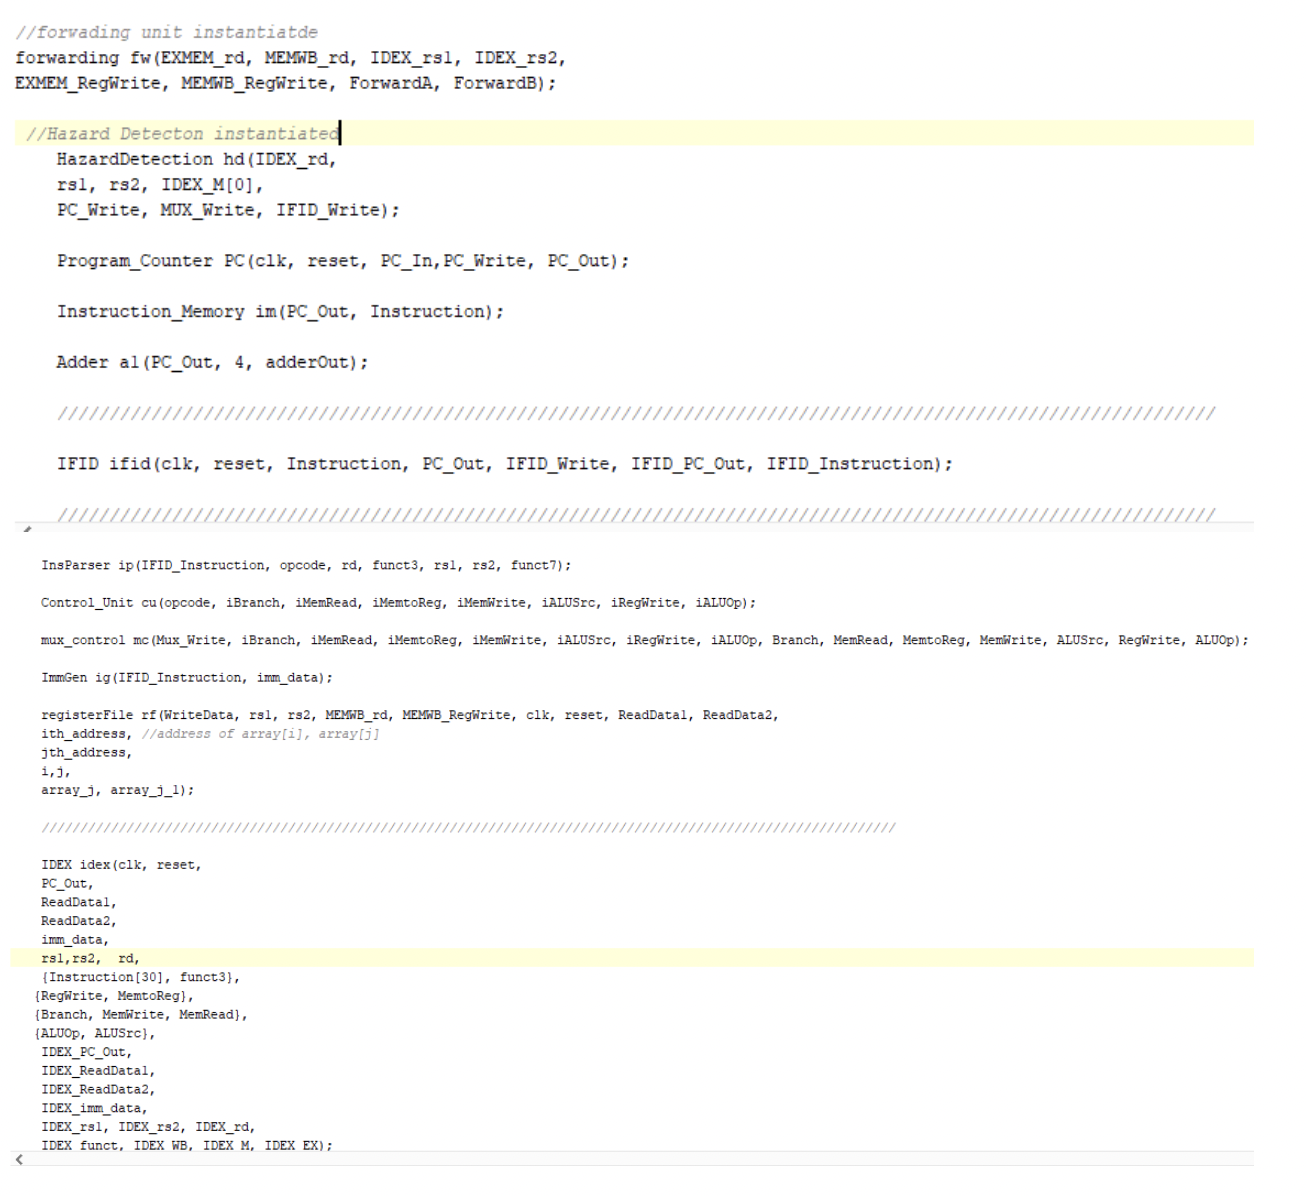
\includegraphics[scale = 0.5]{pipe top 4.png}
\\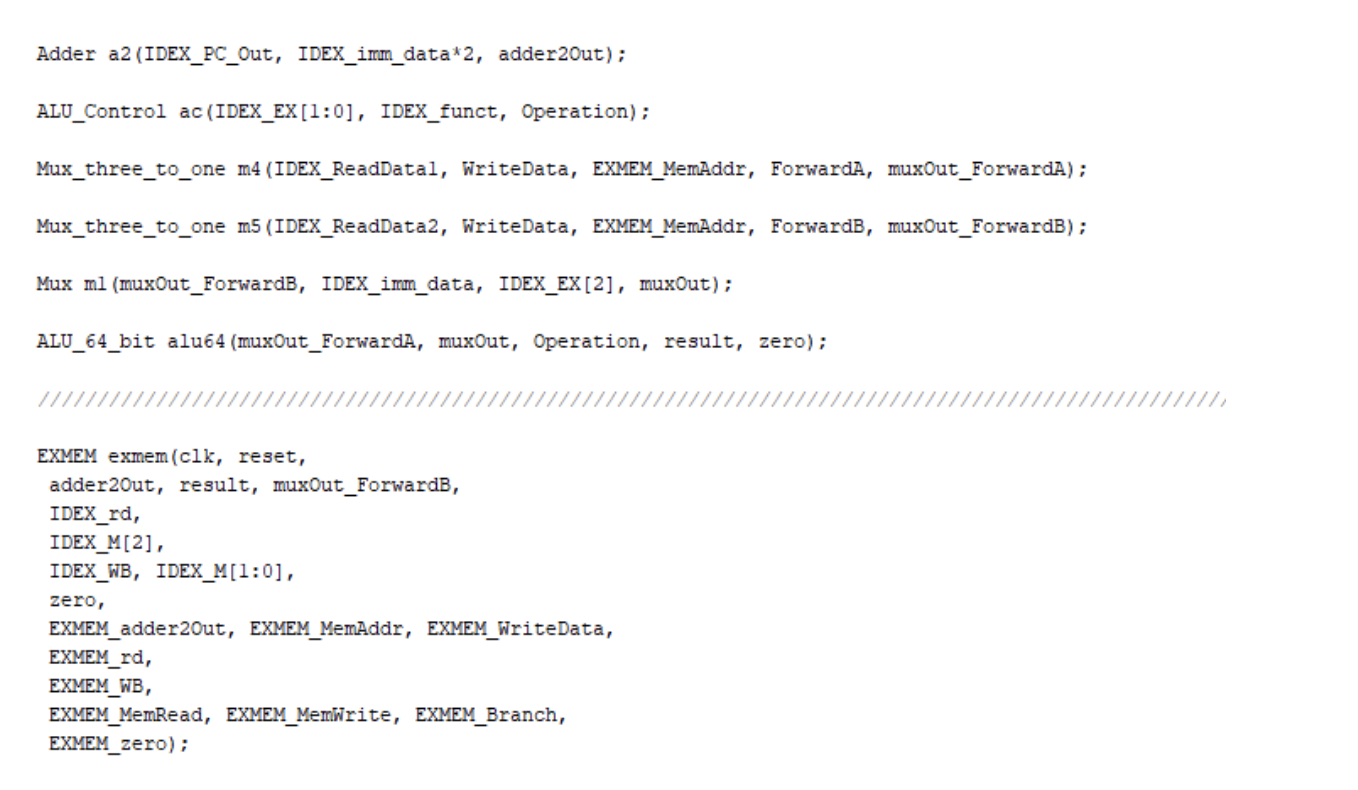
\includegraphics[scale = 0.5]{pipe top 5.png}
\\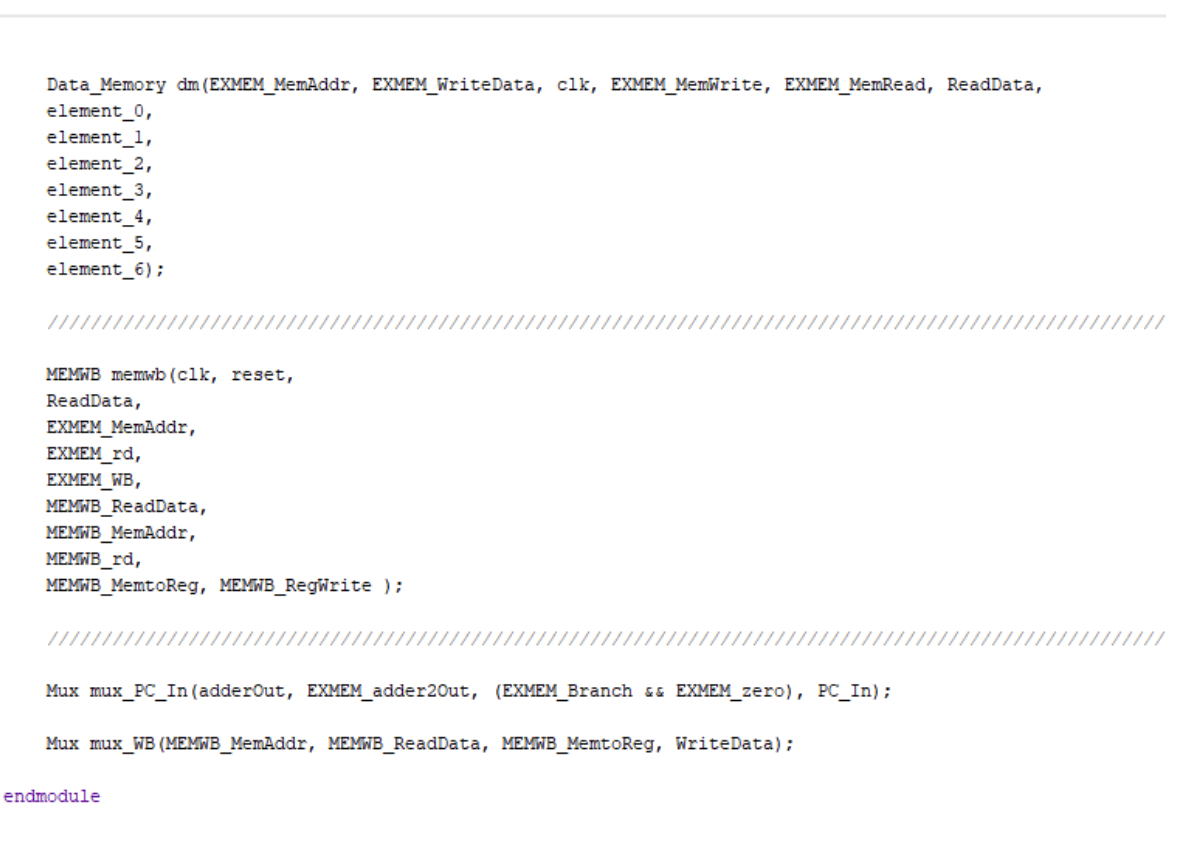
\includegraphics[scale = 0.5]{pipe top 6.png}
\\The test module for this pipelined processor was made as follows:
\\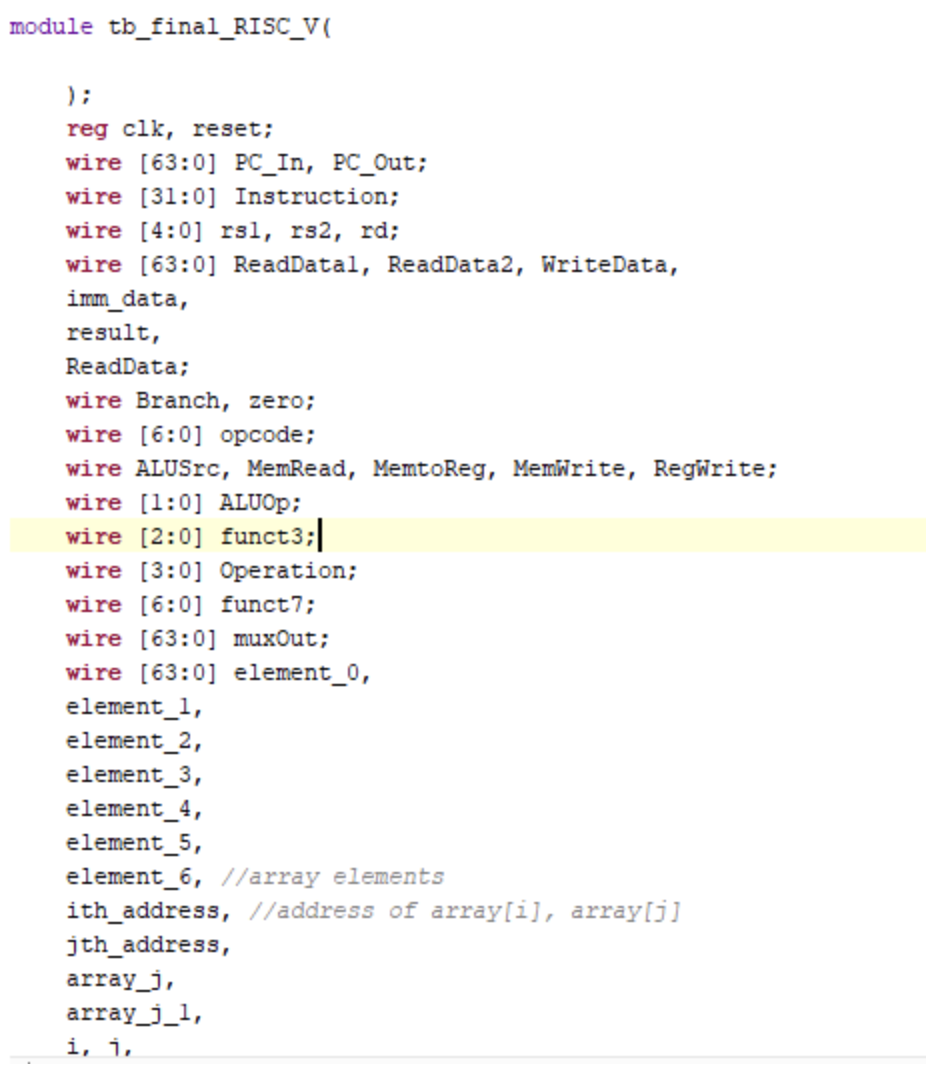
\includegraphics[scale = 0.5]{pipe test 1.png}
\\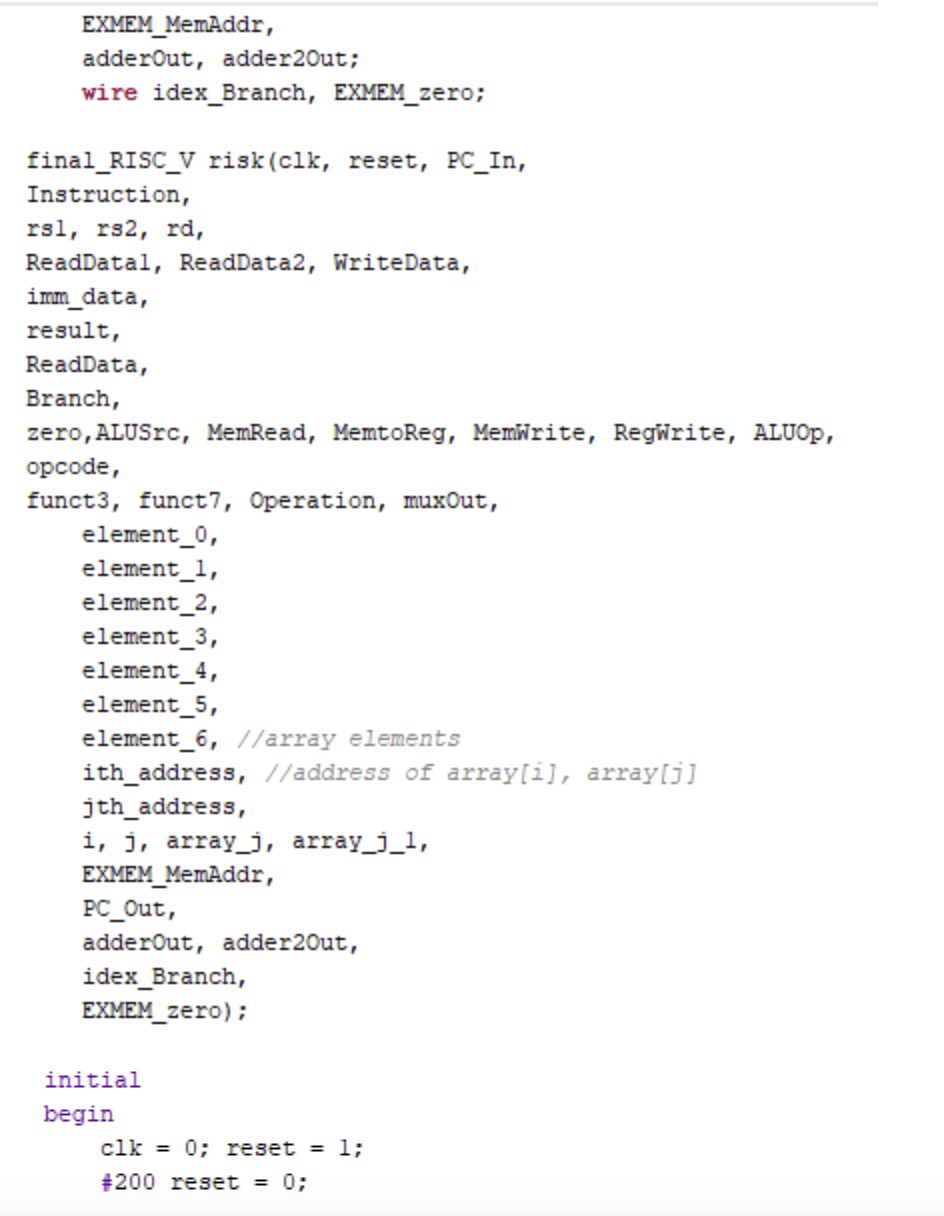
\includegraphics[scale = 0.5]{pipe test 2.png}
\\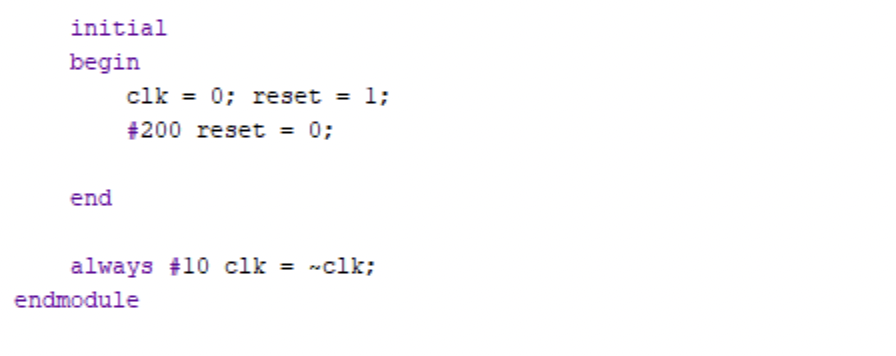
\includegraphics[scale = 0.5]{pipe test 3.png}
\\With this the following EP waves were generated:
\\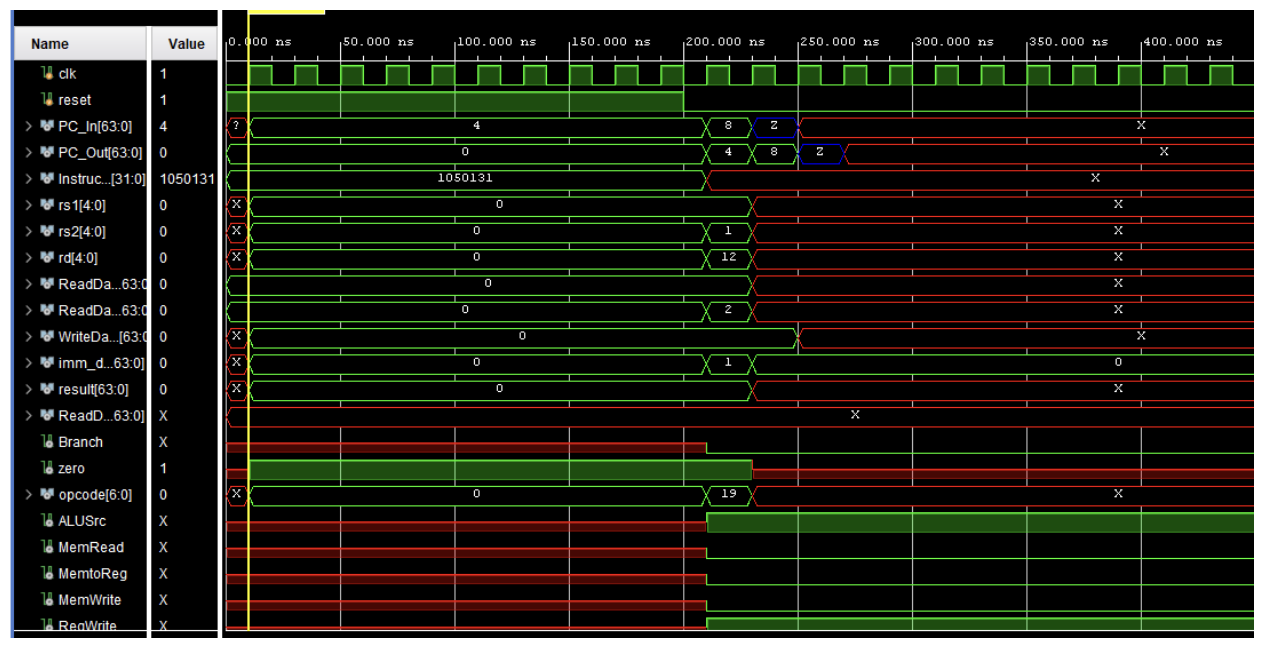
\includegraphics[scale = 0.5]{pipe ep 1.png}
\\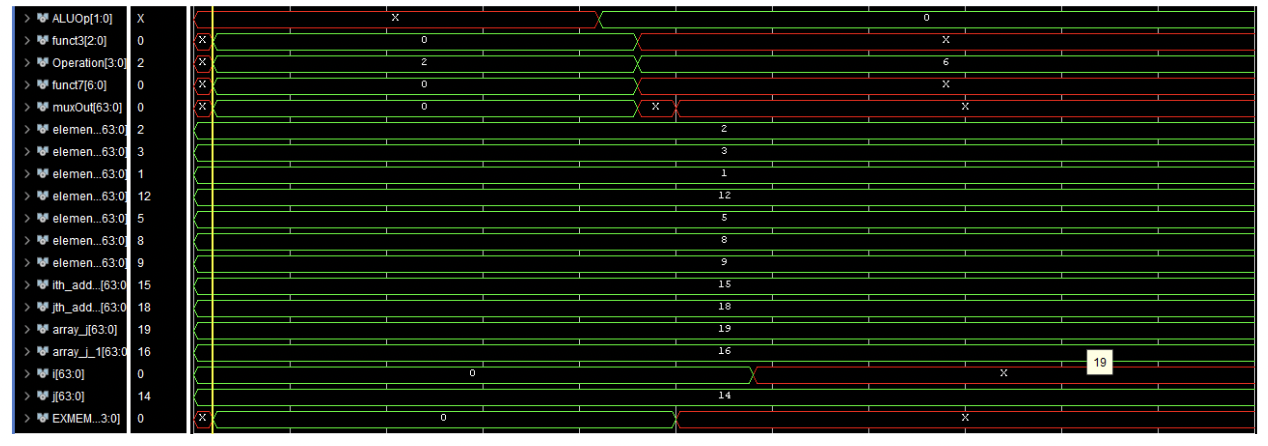
\includegraphics[scale = 0.5]{pipe ep 2.png}
\\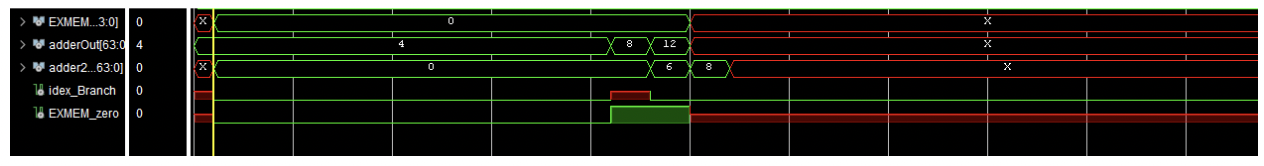
\includegraphics[scale = 0.5]{pipe ep 3.png}
\\Here our processor works for most instructions, but it cannot handle branch instructions. Also when given multiple instruction on the 3rd cycle we started getting some garbage value in PC.
These were the errors that occured but besides that our implemention worked.
\\The code for Intermediate Modules can be found in the appendix.
\section*{Challenges}
The biggest challenge we faced was that our processor couldn't handle branch instructions. 
The code for handling branch instruction was implemented but there was some bug in that code due to which our processor couldn't handle branch instructions.
We tried debugging it but we couldn't fix this issue.
\\The next challeneg we faced was that when given multiple instructions out pipelined processor would stop working on the third cycle and PC would have a garbage value.
We suspect that the forwarding unit may have issues but it was implemented according to the the implemention we covered in class. We werent able to identify and fix any errors in forwarding if there were any.
\vspace{2cm}
\\The work division was as follows:
\begin{itemize}
    \item \textbf{Muhammad Arsalan Hussain:} worked on pipelining single cycle processor and writing sorting algorithm.
    \item \textbf{Muhammad Hashim Memon:} worked on writing assembly code for sorting algorithm.
    \item \textbf{Syed Muhammad Ather Hashmi:} worked on EXMEM Pipline REgister, Forwarding Unit and Hazard Detection Module.
    \item \textbf{Syed Mujtaba Hassan:} worked on writing machine code and debugging.
\end{itemize}

\section*{Conclusions}
For the single cycle processor our implemention worked great.
\\For the pipelined version it worked fine in most instances but had issues in certain conditions.
First the issue we had was that our processor couldnt handle branch instructions even though we implemented it. The next issue was the case of getting garbage value in PC which was another problem we couldn't fix.
\\There are many reasons why the project didn't turn out to be successful. The first issue was the time constraint, debuggng the error was very difficult in the given time specially after adding all the workload from the semester.
The next issue was the issues with verilog, we had a bunch of issues with verilog that we had trouble fixing, debugging is harder in vivado due to not having intellisense.
\\There were also the main issue we had was that we couldn't identify the bug that we were having due to which the project wasn't a success.
\section*{References}
The designs were taken from the following book:
\\\href{http://home.ustc.edu.cn/~louwenqi/reference_books_tools/Computer%20Organization%20and%20Design%20RISC-V%20edition.pdf}{Computer Organization and Design by David A. Patterson and John L. Hennessy}
\section*{Appendices}
The following git repository contains out entire code:
\\\href{https://github.com/mh07607/RISC_V_Processor.git}{\url{https://github.com/mh07607/RISC_V_Processor.git}}
% \href{https://github.com/mh07607/RISC_V_Processor.git}{g}
\end{document}